
\documentclass[12pt]{exam}
\usepackage{amsthm}
\usepackage{libertine}
%\usepackage[utf8]{inputenc}
\usepackage[margin=1in]{geometry}
\usepackage{amsmath,amssymb}
\usepackage{multicol}
\usepackage[shortlabels]{enumitem}
\usepackage{siunitx}
\usepackage{cancel}
\usepackage{graphicx}
\graphicspath{{./}}
\usepackage{pgfplots}
\usepackage{hyperref}
\usepackage{listings}
\usepackage{tikz}
\usepackage{minted}
\def\code#1{\texttt{#1}}
\usepackage{amssymb}
\usepackage{xcolor}
% for plotting
\usepackage{pgfplots}
\pgfplotsset{compat=1.16}
\usepackage{tikz}
\usetikzlibrary{arrows.meta}

\newcommand{\quotebox}[1]
{
  \begin{center}
    \fcolorbox{white}{blue!15!gray!15}{
      \begin{minipage}{0.7\linewidth}\vspace{10pt}
        \center
        \begin{minipage}{0.8\linewidth}{\space\Huge``}{\setlength{\parindent}{1.5em}#1}{\hspace{1.5em}\break\null\Huge\hfill''}
        \end{minipage}
        \smallbreak
      \end{minipage}
    }
\end{center}
}

%\DeclareUnicodeCharacter{2212}{-}


\let\oldemptyset\emptyset
\let\emptyset\varnothing

\hypersetup{
    colorlinks=true,
    linkcolor=blue,
    filecolor=magenta,      
    urlcolor=cyan,
    pdftitle={Overleaf Example},
    pdfpagemode=FullScreen,
    }
    
\urlstyle{same}

\pgfplotsset{width=10cm,compat=1.9}
\usepgfplotslibrary{external}
\tikzexternalize

\newcommand{\class}{Math 415} % This is the name of the course 
\newcommand{\examnum}{Homework-9} % This is the name of the assignment
\newcommand{\examdate}{Nov 20} % This is the due date
\newcommand{\timelimit}{}

\newcommand{\BO}{\mathcal{O}}




\begin{document}
\pagestyle{plain}
\thispagestyle{empty}

\noindent
\begin{tabular*}{\textwidth}{l @{\extracolsep{\fill}} r @{\extracolsep{6pt}} l}
\textbf{\class} & \textbf{Name:} & \textit{Zhenzhao Tu}\\ %Your name here instead, obviously 
\textbf{\examnum} &&\\
\textbf{\examdate} &&\\
\end{tabular*}\\
\rule[2ex]{\textwidth}{2pt}
% --


\section*{Problem 1}
Show that the system $\dot{x} = x-y-x^3$, $\dot{y} = x+y -y^3$ has a periodic solution using Poincar\'e–Bendixson Theorem.
\begin{proof}
	First we can use $(x,y) = (r\cos\theta, r\sin\theta)$ to transform the system into polar coordinates:
	\begin{align*}
		\dot{r} &= r- r^3 -2r^3\cos^2\theta \sin^2\theta\\
		\dot{\theta} &= 1 + \frac{1}{4}r^2\sin 4\theta
	\end{align*}
	To such Poincar\'e–Bendixson Theorem applies, we need to show that $(4)$ condition holds. Now seek two concertric circles with radius $r_{min}$ and $r_{max}$ such that $r_{min} < r < r_{max}$. First, to find $r_{min}$, we require $\dot{r} > 0$ for all $\theta$. This is equivalent to
	\[ \dot{r} = r(1-r^2-2r^2\cos^2\theta\sin^2\theta) > 0 \]
	Thus we have sufficient condition $r < 1/ \sqrt{1+2\cos^2\theta\sin^2\theta}$. Since $\cos^2\theta\sin^2\theta = 1/4$ makes the denominator largest, we have $r_{min} = 1/\sqrt{1+1/2} = \sqrt{2/3}$. Similarly, to find $r_{max}$, we require $\dot{r} < 0$ for all $\theta$. This is equivalent to
	\[ \dot{r} = r(1-r^2-2r^2\cos^2\theta\sin^2\theta) < 0 \]
	Thus we have sufficient condition $r > 1/ \sqrt{1+2\cos^2\theta\sin^2\theta}$. Since $\cos^2\theta\sin^2\theta = 0$ makes the denominator smallest, we have $r_{max} = 1/\sqrt{1+0} = 1$. Thus we have $r_{min} < r < r_{max}$ for all $r$. Now we can apply Poincar\'e–Bendixson Theorem to conclude that there exists a periodic solution.
\end{proof}


\section*{Problem 2}
Consider the system 
\[ \dot{x} = x(1-4x^2 - y^2)- \frac{1}{2}y(1+x), \quad \dot{y} = y(1-4x^2 - y^2)+ 2x(1+x) \]
\begin{enumerate}[(a)]
	\item Show that the origin is an unstable fixed point.\\
	Let $\dot{x} = 0$ and $\dot{y} = 0$, we have $x = 0$ and $y = 0$. Thus the origin is a fixed point. Now we can use linearization to determine the stability of the fixed point. The Jacobian matrix is
	\[ J = \begin{bmatrix}
	1-12x^2-y^2-\frac{1}{2}y & -2xy-\frac{1}{2}(1+x)\\
		8xy + 2+4x & 1-4x^2-3y^2
	\end{bmatrix}_{(0,0)}  = \begin{bmatrix}
		1 & -1/2\\
		2 & 1
	\end{bmatrix} \]
	The eigenvalues of $J$ are $\lambda_1 = 1 + i$ and $\lambda_2 = 1 - i$. Since the real part of the eigenvalues are positive, the origin is an unstable fixed point.
	\item By considering $\dot{V}$, where $V(x,y) = (1-4x^2-y^2)^2$, show that all trajectories approach the ellipse $4x^2 + y^2 = 1$ as $t \to \infty$.\\
	Let's take $\dot{V}$:
	\[ \dot{V} = \frac{\partial V}{\partial x}\dot{x} + \frac{\partial V}{\partial y}\dot{y} \]
	then we plugin the $\dot{x}$, $\dot{y}$, $\frac{\partial V}{\partial x}$, $\frac{\partial V}{\partial y}$ into the equation above. 
	\begin{align}
		\dot{x} &= x(1-4x^2 - y^2)- \frac{1}{2}y(1+x)\\
		\dot{y} &= y(1-4x^2 - y^2)+ 2x(1+x)\\
		\frac{\partial V}{\partial x} &= -8x(1-4x^2-y^2)\\
		\frac{\partial V}{\partial y} &= -2y(1-4x^2-y^2)
	\end{align}
	Thus we have
	\begin{align*}
		\dot{V} &= -8x^2(1-4x^2-y^2)^2 - 2y^2(1-4x^2-y^2)^2 - \frac{1}{2}y(1+x)(1-4x^2-y^2) \\
			& \qquad + 2x(1+x)(1-4x^2-y^2) \\
			& = -4(-1+4x^2+y^2)^2(4x^2+y^2)
	\end{align*}
	Now we can see that $\dot{V} = 0$ if $4x^2 + y^2 = 1$. That indicated that the ellipse $4x^2 + y^2 = 1$ is a limit cycle. If we consider $4x^2 + y^2 < 1$, then $\dot{V} < 0$ and if $4x^2 + y^2 > 1$, then $\dot{V} < 0$. Thus all trajectories approach the ellipse $4x^2 + y^2 = 1$ as $t \to \infty$.
\end{enumerate}

\section*{Problem 3}
Consider the equation $\ddot{x} + \mu f(x) \dot{x} + x=0$, where 
\[ f(x) = \begin{cases}
	1, & |x| \geq 1\\
	-1, & |x| < 1
\end{cases} \]

\begin{enumerate}[(a)]
	\item Let $x= -\mu \dot{y}$, then plug it into the equation above, we have
	\[ \ddot{x} + \mu f(x) \dot{x} - \mu \dot{y} = 0 \]
	then if we intgrate the equation from both sides, we have
	\[ \int \ddot{x}  = \int  \mu \dot{y}- \mu f(x) \dot{x} \]
	\[ \dot{x} = \mu y - \mu (F(x) + C) \]
	where $F(x)$ is the antiderivative of $f(x)$. Now we have a system
	\[ \begin{cases}
		\dot{x} = \mu y - \mu (F(x) + C)\\
		\dot{y} = -\frac{1}{\mu}x
	\end{cases} \]
	When $|x| \leq 1$, we have $f(x) = -1$, thus $F(x) = -x$ and the system becomes	
	\[ \begin{cases}
		\dot{x} = \mu y + \mu x - \mu C\\
		\dot{y} = -\frac{1}{\mu}x
	\end{cases} \]
	where $C$ is a constant. When $|x| > 1$, we have $f(x) = 1$, thus $F(x) = x$ and the system becomes
	\[ \begin{cases}
		\dot{x} = \mu y - \mu x + \mu C\\
		\dot{y} = -\frac{1}{\mu}x
	\end{cases} \]
	where $C$ is a constant.
	Now we choose $C = 2$ when $x \leq -1$ and $C = -2$ when $x \geq 1$. Then we have
	\[ F(x) = \begin{cases}
		x+2, & x \leq -1\\
		-x, & |x|\leq 1\\
		x-2, & x \geq 1
	\end{cases} \]


	\item The nullclines plot for $F(x)$ is shown below:

		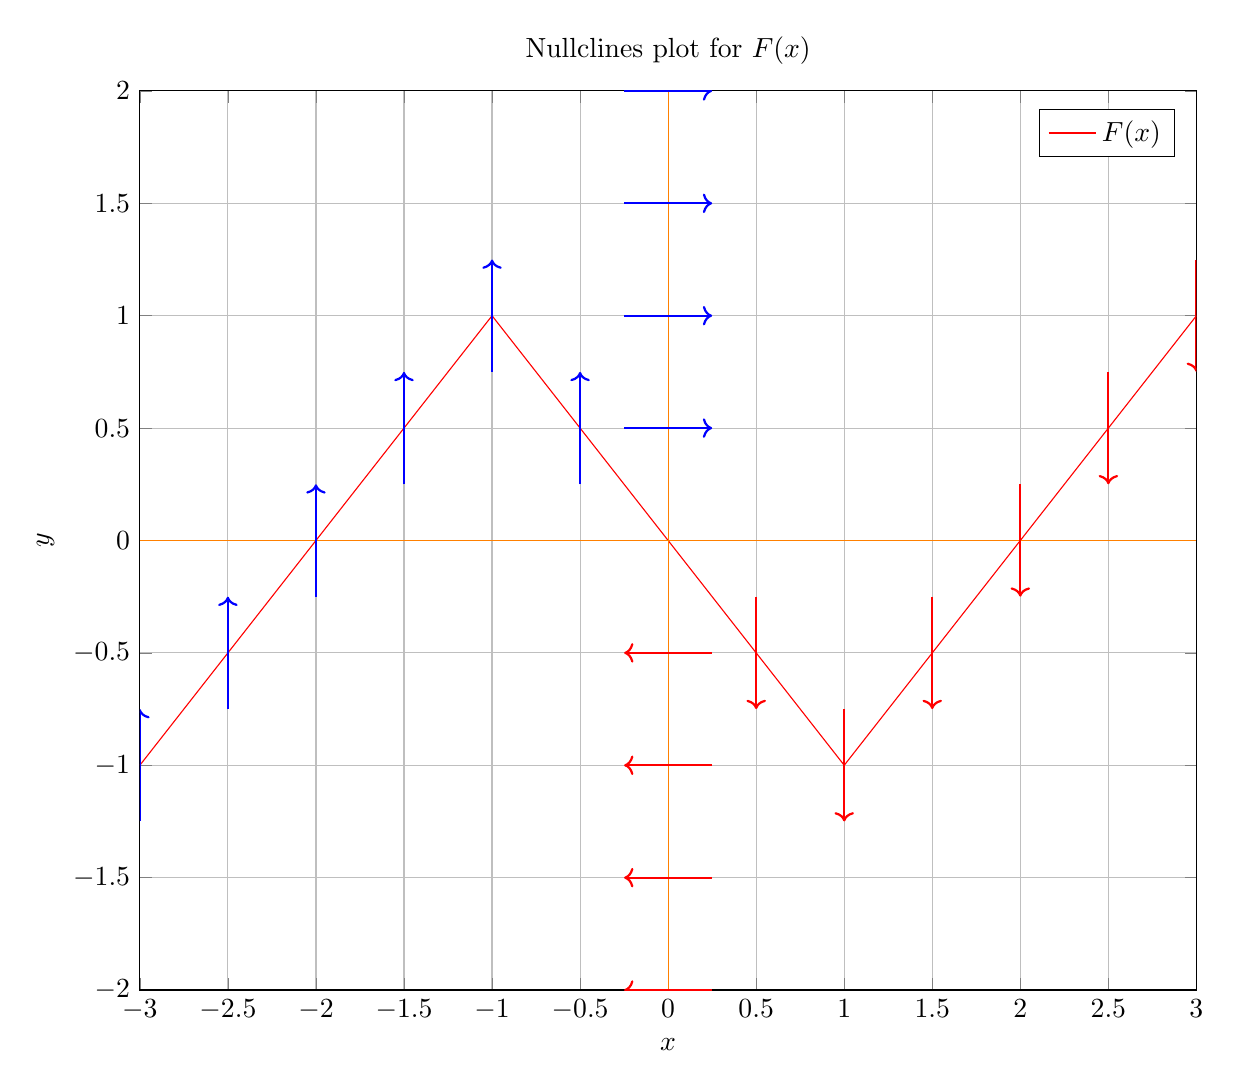
\begin{tikzpicture}
		\begin{axis}[
			title={Nullclines plot for $F(x)$},
			xlabel={$x$},
			ylabel={$y$},
			xmin=-3, xmax=3,
			ymin=-2, ymax=2,
			grid=both,
			width=15cm,
			height=13cm
			]
		\addplot[domain=-3:-1, samples=100, color=red]{x+2};
		\addplot[domain=-1:1, samples=100, color=red]{-x};
		\addplot[domain=1:3, samples=100, color=red]{x-2};
		% add blue horizontal line y=0
		\addplot[domain=-3:3, samples=100, color=orange]{0};
		% add blue vertical line x=0
		\addplot[orange, domain=-2:2, samples=100] coordinates {(0,-2) (0,2)};

		% add vector from (0.5, -0.25) to (0.5, -0.75)
		\addplot[->, thick, color=red] coordinates {(0.5, -0.25) (0.5, -0.75)};
		% add vector from (1, -0.75) to (1, -1.25)
		\addplot[->, thick, color=red] coordinates {(1, -0.75) (1, -1.25)};
		% add vector from (1.5, -0.25) to (1.5, -0.75)
		\addplot[->, thick, color=red] coordinates {(1.5, -0.25) (1.5, -0.75)};
		% add vector from (2, 0.25) to (2, -0.25)
		\addplot[->, thick, color=red] coordinates {(2, 0.25) (2, -0.25)};
		% add vector from (2.5, 0.75) to (2.5, 0.25)
		\addplot[->, thick, color=red] coordinates {(2.5, 0.75) (2.5, 0.25)};
		% add vector from (3, 1.25) to (3, 0.75)
		\addplot[->, thick, color=red] coordinates {(3, 1.25) (3, 0.75)};

		% add vector from (-0.5, 0.25) to (-0.5, 0.75) with blue color
		\addplot[->, thick, color=blue] coordinates {(-0.5, 0.25) (-0.5, 0.75)};
		% add vector from (-1, 0.75) to (-1, 1.25) with blue color
		\addplot[->, thick, color=blue] coordinates {(-1, 0.75) (-1, 1.25)};
		% add vector from (-1.5, 0.25) to (-1.5, 0.75) with blue color
		\addplot[->, thick, color=blue] coordinates {(-1.5, 0.25) (-1.5, 0.75)};
		% add vector from (-2, -0.25) to (-2, 0.25) with blue color
		\addplot[->, thick, color=blue] coordinates {(-2, -0.25) (-2, 0.25)};
		% add vector from (-2.5, -0.75) to (-2.5, -0.25) with blue color
		\addplot[->, thick, color=blue] coordinates {(-2.5, -0.75) (-2.5, -0.25)};
		% add vector from (-3, -1.25) to (-3, -0.75) with blue color
		\addplot[->, thick, color=blue] coordinates {(-3, -1.25) (-3, -0.75)};
		
		% add vector from (-0.25, 0.5) to (0.25, 0.5) with blue color
		\addplot[->, thick, color=blue] coordinates {(-0.25, 0.5) (0.25, 0.5)};
		% add vector from (-0.25, 1) to (0.25, 1) with blue color
		\addplot[->, thick, color=blue] coordinates {(-0.25, 1) (0.25, 1)};
		% add vector from (-0.25, 1.5) to (0.25, 1.5) with blue color
		\addplot[->, thick, color=blue] coordinates {(-0.25, 1.5) (0.25, 1.5)};
		% add vector from (-0.25, 2) to (-0.25, 2) with blue color
		\addplot[->, thick, color=blue] coordinates {(-0.25, 2) (0.25, 2)};

		% add vector from (0.25, -0.5) to (-0.25, -0.5) with red color
		\addplot[->, thick, color=red] coordinates {(0.25, -0.5) (-0.25, -0.5)};
		% add vector from (0.25, -1) to (-0.25, -1) with red color
		\addplot[->, thick, color=red] coordinates {(0.25, -1) (-0.25, -1)};
		% add vector from (0.25, -1.5) to (-0.25, -1.5) with red color
		\addplot[->, thick, color=red] coordinates {(0.25, -1.5) (-0.25, -1.5)};
		% add vector from (0.25, -2) to (0.25, -2) with red color
		\addplot[->, thick, color=red] coordinates {(0.25, -2) (-0.25, -2)};



		\legend{$F(x)$}
		\end{axis}
		\end{tikzpicture}


	\item Consider a random point near the origin, say $(x_0, y_0) = (0.5, 0.5)$. Then we have our system
		\[ \begin{cases}
			\dot{x} = \mu (\frac{1}{2} + \frac{1}{2}) \\
			\dot{y} = -\frac{1}{2\mu}
		\end{cases} \]
		Now since $\mu \gg 1$, $\dot{x} \gg \dot{y}$. Thus the trajectory will move to the right very fast. When the trajectory reaches around $(2.4, 0.5)$ the system will switch to
		\[ \begin{cases}
			\dot{x} = \mu (2.4 - 0.5 - 2) \\
			\dot{y} = -\frac{1}{2.6\mu}
		\end{cases} \]
		Then, $\dot{x}$ and $\dot{y}$ will be very small and the trajectory will move to the left down very slowly. Thus the trajectory will repeat this process and oscillate around the origin as shown in the plot below:
		\begin{figure}[H]
			\centering
			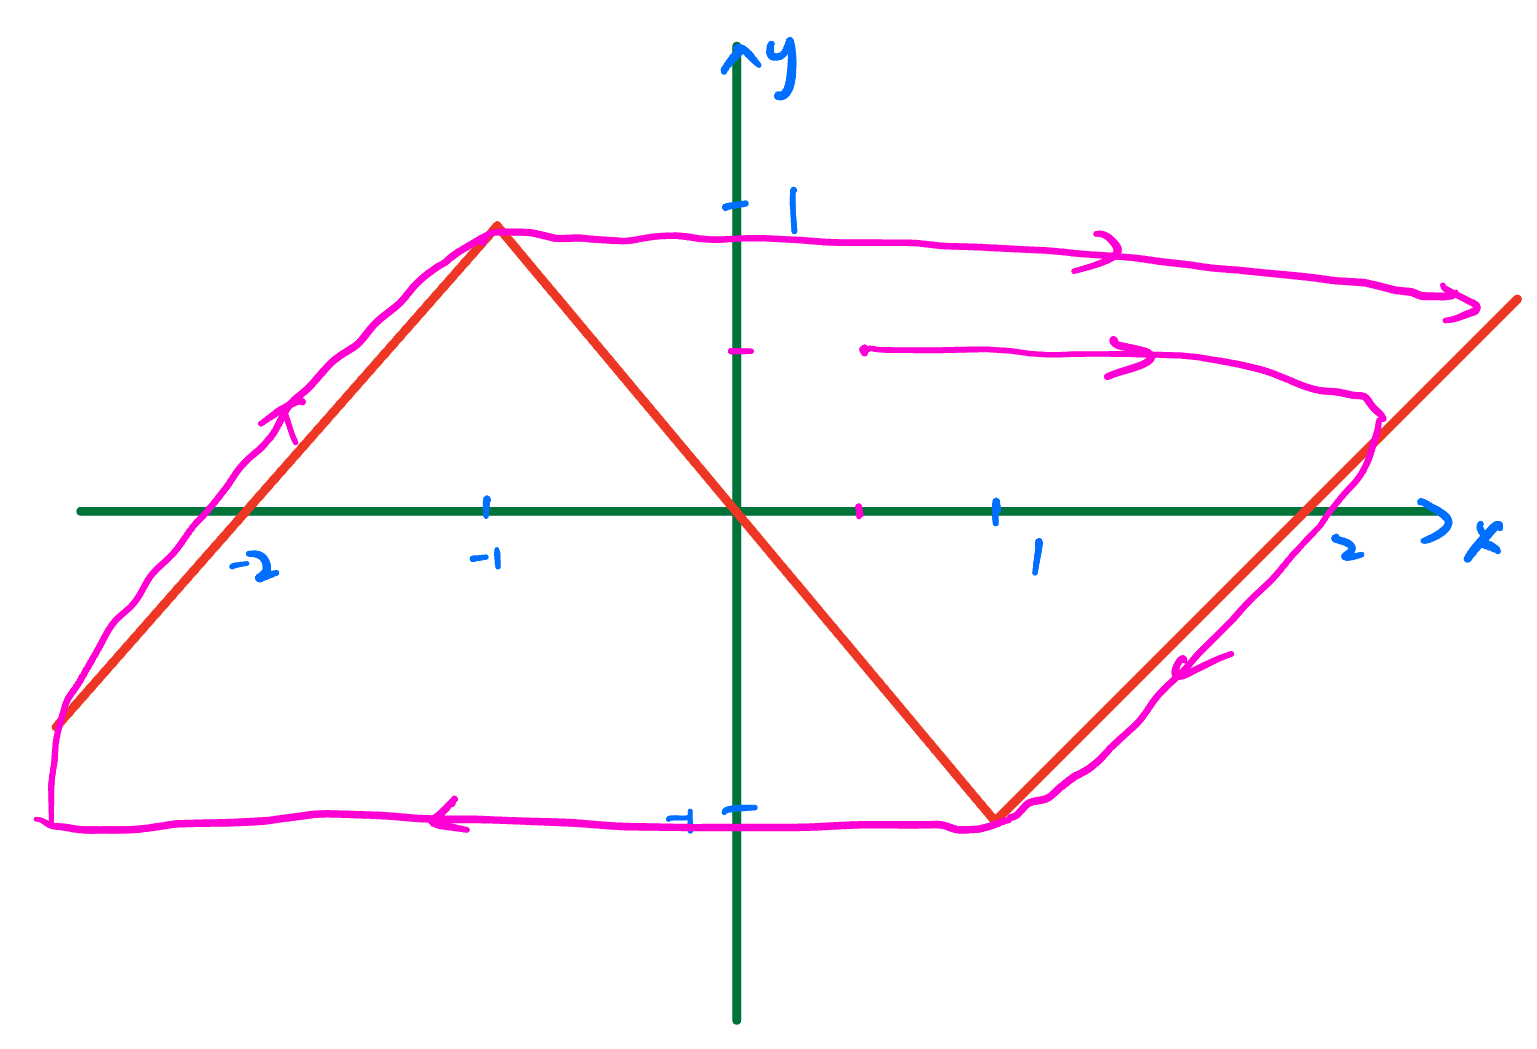
\includegraphics[width=0.8\linewidth]{3c.jpeg}
			\caption{Trajectory of the system}
		\end{figure}









\end{enumerate}

\end{document}

